\newpage

\addcontentsline{toc}{section}{Введение}
\section*{\centering{\uppercase{Введение}}}

В последние десятилетия концепция «пользовательского контента» приобрела широкое распространение, а с развитием интернет-технологий появились проекты, в которых пользователи могут активно взаимодействовать друг с другом в рамках виртуальных платформ. Одним из ярких примеров таких проектов является r/Place — социальный эксперимент, проведённый на платформе Reddit, в котором пользователи могли размещать пиксели на общей картине, создавая таким образом коллективное произведение искусства. Этот проект стал не только местом для творческого самовыражения, но и уникальной возможностью для наблюдения за коллективным поведением и взаимодействием пользователей в реальном времени. Вдохновленная этим экспериментом, игра Pixel Wars представляет собой аналог r/Place, но с усовершенствованиями в механике взаимодействия, такие как система рейтингов и должностей.

За последние несколько лет разработка многопользовательских онлайн-игр и платформ, которые обеспечивают взаимодействие пользователей в реальном времени, стала важной частью исследований в области геймдизайна и программирования.

Целью данной курсовой работы является разработка многопользовательской игры Pixel Wars, аналогичной r/Place, с уникальной игровой механикой и интерфейсом, предоставляющим пользователю возможность взаимодействовать с другими игроками в реальном времени. В процессе работы будут исследованы аспекты проектирования интерфейсов, работы с базами данных, а также реализована система взаимодействия между игроками, поддерживающая динамичные изменения в игровом мире.

При проектировании игры использовались принципы модульности, гибкости интерфейса и оптимизации работы серверной части приложения. Основное внимание было уделено разработке механики взаимодействия пользователей с картой.

Для достижения данной цели предусмотрены следующие задачи:
\begin{itemize}
    \item Анализ аналогов
    \item Проектирование архитектуры
    \item Реализация серверной части
    \item Разработка пользовательского интерфейса
    \item Введение системы модерации
    \item Тестирование
\end{itemize}

\newpage

\sectionuppercase{Обзор существующих аналогов}

\subsection{Оригинальный r/Place}

\begin{figure}[H]
    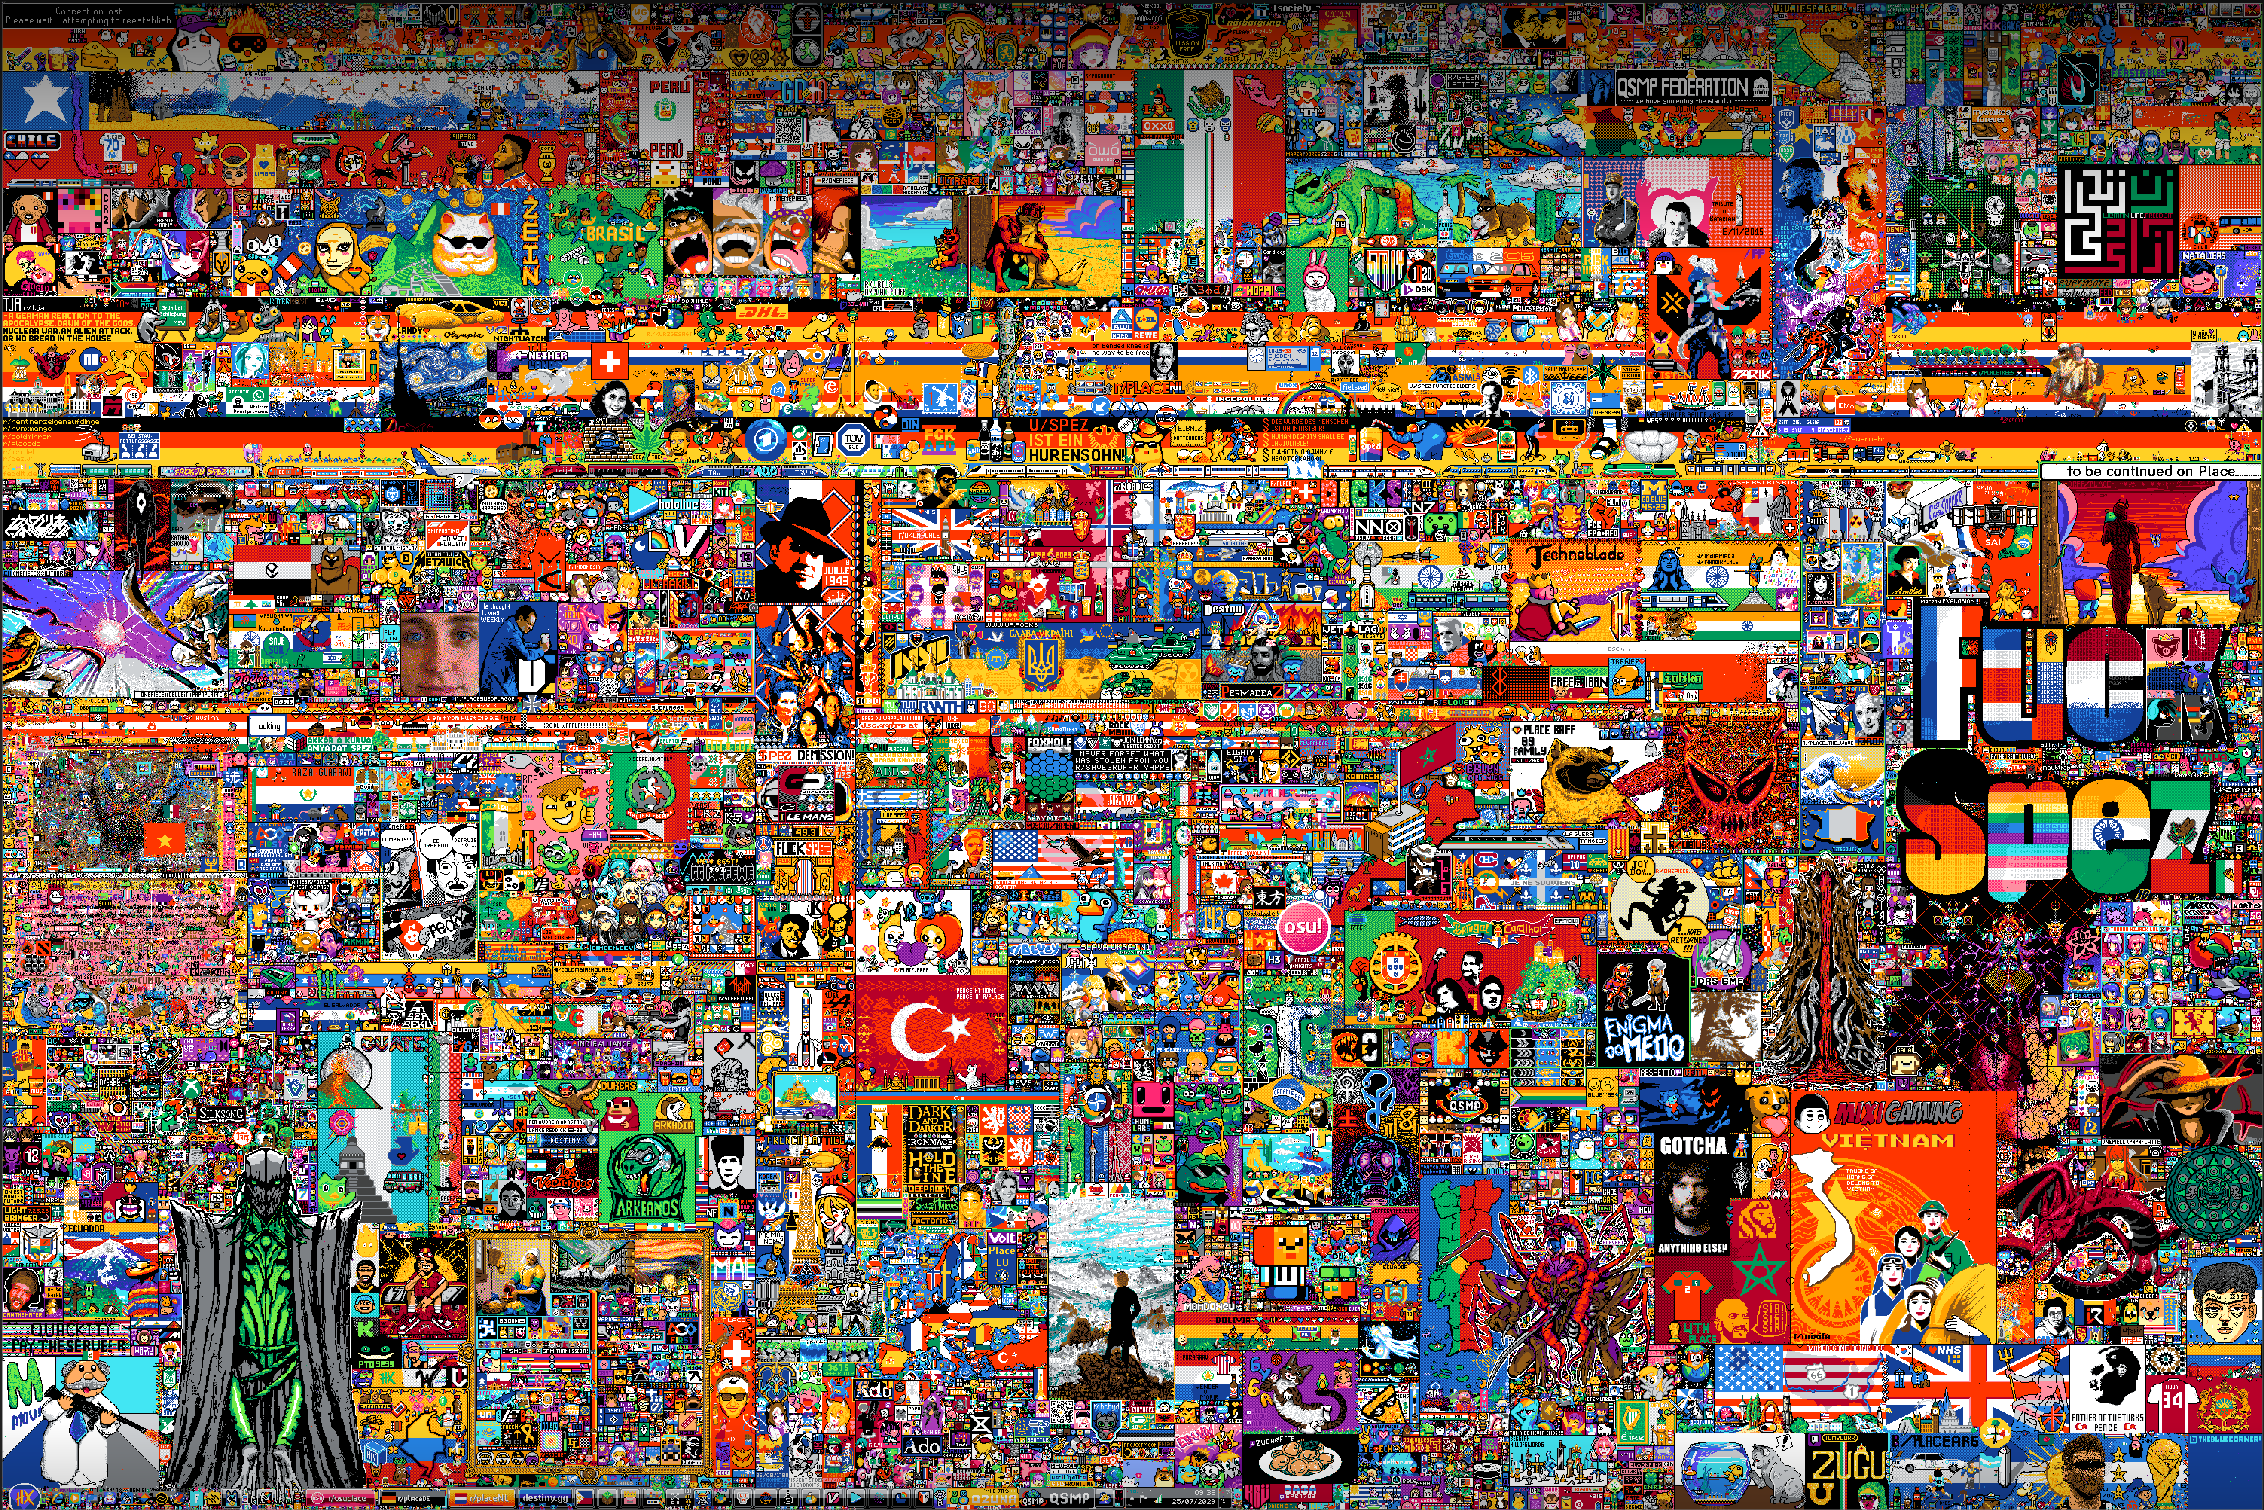
\includegraphics[width=\textwidth]{rplace.png}
    \caption{Финальный холст r/Place 2023}
\end{figure}

r/Place --- это социальный эксперимент, проведённый платформой Reddit в 2017 году, который позволил пользователям размещать пиксели на огромной сетке размером 1000x1000 пикселей \cite{rplace}. Каждому участнику предоставлялся ограниченный выбор цветов для одного пикселя, который можно было разместить на картине. Однако, через некоторое время, любой другой пользователь мог изменить или удалить размещённый пиксель. Это создавалось условия для динамичного взаимодействия, конкуренции и коллективного творчества, так как участники должны были защищать свои изображения от «вандалов» и сражаться за территорию на картине.

Основной целью r/Place было изучение коллективного поведения и взаимодействия пользователей в условиях ограниченных ресурсов. Проект позволил наблюдать, как участники организуют коллективные усилия для создания и сохранения изображений, а также как возникают временные альянсы и конфликты. Созданная карта стала живым примером коллективного разума, где каждый пиксель был важен для общего результата.

Социальный эксперимент стал значимой вехой в изучении цифровых сообществ, показав, как большое количество людей может взаимодействовать в реальном времени, создавая совместное произведение искусства. В 2022 году был проведён повторный запуск r/Place, который использовал улучшенную механику и привлёк ещё больше участников.

\subsection{PixelPlace.io}

\begin{figure}[H]
    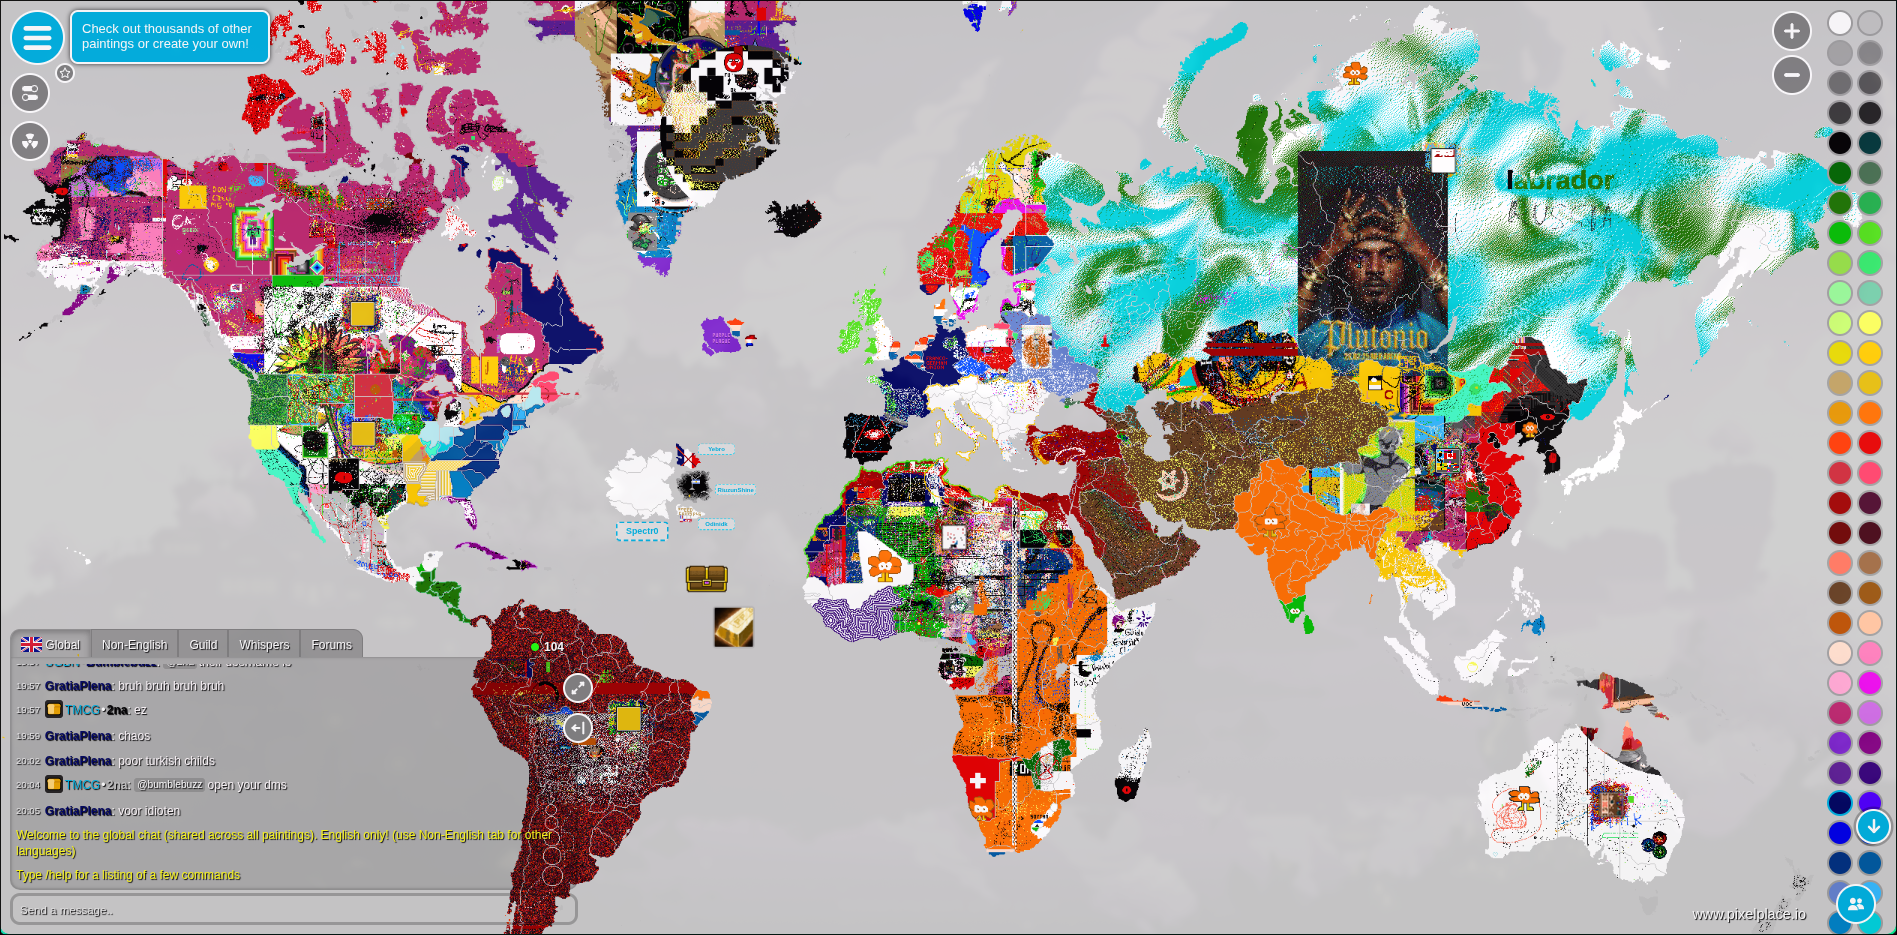
\includegraphics[width=\textwidth]{pixelplace.png}
    \caption{Фрагмент холста и интерфейса PixelPlace.io}
\end{figure}

PixelPlace.io --- это многопользовательская онлайн-игра, вдохновлённая концепцией r/Place, в которой пользователи могут размещать пиксели на общем холсте в реальном времени \cite{pixelplace}. В отличие от оригинального проекта Reddit, данное приложение включает элементы геймификации и более развитую социальную инфраструктуру.

На холсте PixelPlace.io пользователи могут рисовать изображения, координируясь с другими игроками через встроенный чат. Уникальной особенностью платформы является наличие системы прокачки: за размещение пикселей игрок получает опыт, увеличивает уровень и может открывать новые возможности. Интерфейс позволяет отслеживать свою статистику и рейтинг, что стимулирует участие в долгосрочной игровой активности.

Игра предлагает несколько серверов (регионов), каждый из которых имеет свой отдельный холст. Введены механизмы защиты от вандализма --- игроки могут "замораживать"\ пиксели, а также использовать шаблоны, чтобы совместными усилиями воспроизводить изображения. Администрация поддерживает систему модерации и следит за соблюдением правил.

В результате, PixelPlace.io развивает идеи r/Place, превращая коллективное рисование в полноценную соревновательную игру с элементами RPG, рейтингов и кооперативных миссий. Благодаря своей гибкой системе взаимодействия, прогрессии и визуальной составляющей, этот проект стал заметным явлением в жанре многопользовательских пиксельных игр.

\subsection{PixelCanvas.io}

\begin{figure}[H]
    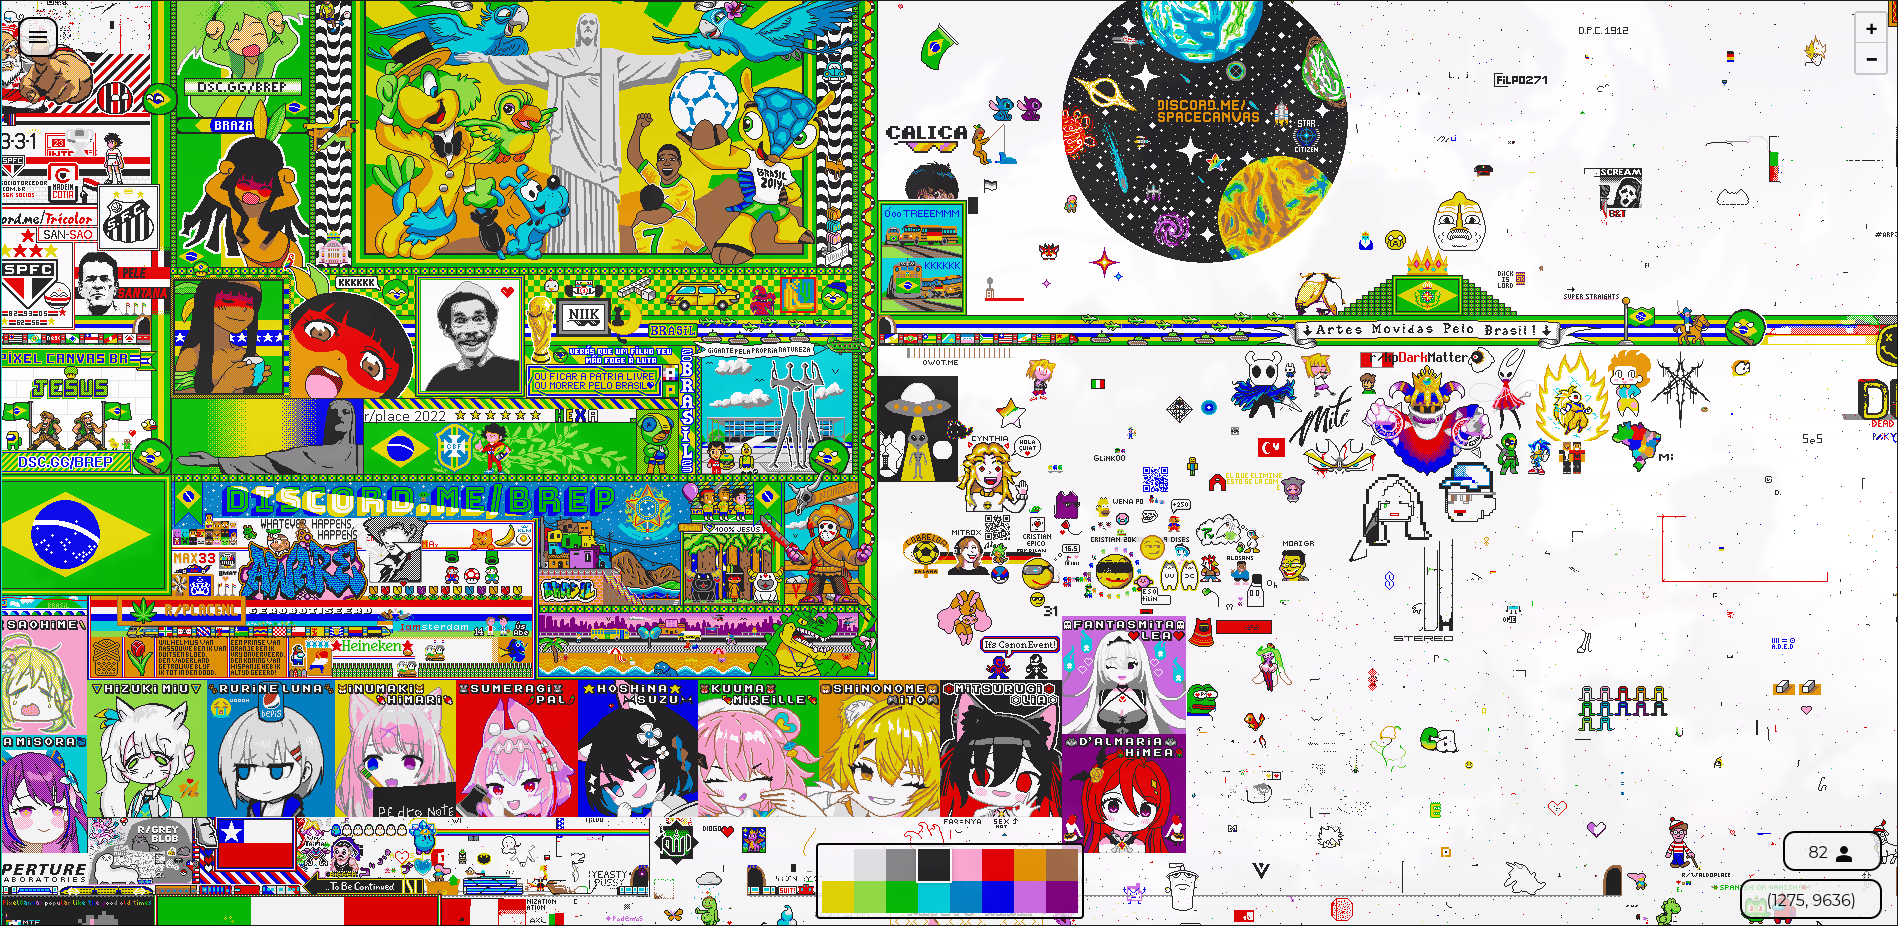
\includegraphics[width=\textwidth]{pixelcanvas.png}
    \caption{Фрагмент холста PixelCanvas.io}
\end{figure}

PixelCanvas.io --- это онлайн-платформа для коллективного рисования, во многом вдохновлённая оригинальным r/Place, но реализованная в более открытом и гибком формате \cite{pixelcanvas}. Данный проект предоставляет пользователям возможность закрашивать пиксели на практически бесконечном холсте, поддерживая масштабные рисунки и долговременные коллаборации.

Ключевой особенностью PixelCanvas.io является масштабность: пользователи могут свободно перемещаться по огромной карте, создавая изображения в любом месте. Система координат позволяет точно размещать шаблоны, что делает платформу удобной для реализации сложных изображений и коллективных проектов. Каждый пиксель можно установить с заданной задержкой, что формирует основу для соревновательного взаимодействия между группами игроков.

Также в игре поддерживается загрузка и наложение шаблонов изображений, что облегчает организацию крупных проектов. Пользователи часто координируются через внешние чаты и форумы. Несмотря на отсутствие формальной системы уровней или рейтингов, активные сообщества создают неофициальные альянсы, соревнуются за территорию и организуют защиту своих работ.

\newpage
\sectionuppercase{Архитектура приложения}

Приложение Pixel Wars построено по клиент-серверной архитектуре, что позволяет реализовать многопользовательское взаимодействие в реальном времени. Данная архитектура обеспечивает централизованное управление игрой, синхронизацию состояния холста, а также упрощает реализацию модерации и системы рейтингов.

Приложение состоит из следующих логических компонентов:
\begin{enumerate}
    \item
          \textbf{Клиетская часть.} Отвечает за отображение интерфейса пользователю, приём его команд (выбор цвета, установка пикселя), а также получение данных с сервера (текущее состояние холста, обновления, сообщения,
          рейтинг и т.д.). Все действия игрока отправляются на сервер, где
          проходят проверку и обработку.

    \item
          \textbf{Серверная часть.} Выполняет обработку всех действий, поступающих от клиентов. Основные функции сервера:
          \begin{itemize}
              \item обновление состояния общей карты;
              \item ведение логов, хранение статистики;
              \item поддержка сессий игроков;
              \item управление таймером;
              \item выполнение модераторских команд (изменение статуса пользователя).
          \end{itemize}

    \item
          \textbf{База данных.} Сервер взаимодействует с базой данных, в которой хранятся:
          \begin{itemize}
              \item информация о пользователях (логины, пароли, статус);
              \item текущее состояние холста (цвета и координаты всех пикселей);
              \item история действий.
          \end{itemize}
\end{enumerate}

\newpage

\section{Технологии программирования, используемые для решения
  поставленных задач}

Здесь мы рассмотрим, какие технологии программирования были
выбраны и по какой причине выбор был именно таким.

\subsection{Язык программирования Java}

\begin{figure}[H]
    \centering
    
\includegraphics[width=0.5\textwidth]{java.png}
    \caption{Java}
\end{figure}

Язык программирования Java является объектно-ориентированным языком, разработанным компанией Sun Microsystems и в настоящее время поддерживаемым корпорацией Oracle. Java обеспечивает высокий уровень абстракции, платформенную независимость и безопасность, что делает его одним из самых популярных языков в мире.

Одним из основных преимуществ Java является его независимость от платформы, достигаемая благодаря использованию виртуальной машины Java (JVM), которая исполняет байт-код, одинаковый для всех операционных систем. Это свойство позволяет создавать переносимые приложения без необходимости модификации исходного кода.

Java поддерживает основные принципы объектно-ориентированного программирования, такие как наследование, инкапсуляция, полиморфизм и абстракция. Эти особенности обеспечивают высокую модульность и повторное использование кода. \cite{java}

В рамках разработки игры Pixel Wars язык Java был выбран как основной инструмент программирования благодаря следующим преимуществам:
\begin{itemize}
    \item наличие обширной стандартной библиотеки, включающей средства для сетевого взаимодействия, работы с потоками, графическим интерфейсом и структурами данных;
    \item развитая экосистема, включающая библиотеки и фреймворки, ускоряющие процесс разработки;
    \item встроенная система управления памятью с автоматическим сборщиком мусора, упрощающая разработку и снижает вероятность ошибок, связанных с управлением ресурсами;
    \item высокая читаемость и строгая типизация, что способствует написанию надёжного и легко сопровождаемого кода.
\end{itemize}

В процессе разработки проекта с использованием Java были реализованы следующие компоненты: взаимодействие с серверной частью через RESTful API, обработка пользовательских действий и реализация механизма обновления состояния в реальном времени.

Таким образом, использование языка Java в проекте позволило обеспечить кроссплатформенность, надёжность и структурированность разрабатываемого программного продукта.

\subsection{Фреймворк Spring}

\begin{figure}[H]
    \centering
    
\includegraphics[width=0.75\textwidth]{spring.png}
    \caption{Spring Framework}
\end{figure}

Spring --- это мощный и гибкий фреймворк с открытым исходным кодом для разработки корпоративных и веб-приложений на языке Java. Благодаря своей модульной структуре, высокой производительности и удобству масштабирования, Spring широко применяется при создании распределённых и высоконагруженных систем, включая веб-сервисы и многопользовательские онлайн-платформы.

Одной из ключевых особенностей Spring является внедрение зависимостей (Dependency Injection), которое способствует слабой связанности компонентов приложения и облегчает их тестирование, повторное использование и расширение. Фреймворк построен по принципу инверсии управления (Inversion of Control), где управление жизненным циклом объектов осуществляется специальным контейнером.

В проекте Pixel Wars фреймворк Spring используется для реализации серверной части приложения, обеспечивающей работу с пользователями, обработку запросов, взаимодействие с базой данных и реализацию защитных механизмов.

В процессе разработки были использованы следующие модули Spring:
\begin{itemize}
    \item Spring Boot --- модуль, предназначенный для упрощения конфигурации и быстрой инициализации проекта. Он предоставляет встроенный сервер и автоматическую настройку компонентов, что позволило сосредоточиться на реализации логики приложения;

    \item Spring Web --- модуль, реализующий обработку HTTP-запросов, маршрутизацию, и построение RESTful API. С его помощью реализовано взаимодействие клиентской и серверной частей, включая передачу данных о пикселях, рейтингах и действиях игроков;

    \item Spring Data --- модуль для работы с базой данных с использованием объектно-реляционного отображения. Он позволяет создавать репозитории и взаимодействовать с таблицами базы данных через Java-классы, что упрощает реализацию слоя доступа к данным;

    \item Spring Security --- модуль, обеспечивающий защиту приложения. В проекте он используется для реализации регистрации, аутентификации и авторизации пользователей, а также ограничения доступа к защищённым ресурсам в зависимости от роли (обычный игрок, модератор и т.д.).
\end{itemize}

Использование Spring позволило добиться высокой скорости обработки запросов, надёжности и масштабируемости серверной части. Благодаря модульной архитектуре фреймворка, разработка велась по принципу разделения ответственности, что улучшило структуру проекта и упростило поддержку и развитие функционала. \cite{spring}

\subsection{База данных PostgreSQL}

\begin{figure}[H]
    \centering
    
\includegraphics[width=0.75\textwidth]{postgresql.png}
    \caption{PostgreSQL}
\end{figure}

Для хранения данных в проекте Pixel Wars используется система управления базами данных PostgreSQL. Это современное, высокопроизводительное и надёжное решение, широко применяемое для создания отказоустойчивых и масштабируемых серверных приложений.

Структура базы данных сформирована в соответствии с предметной областью проекта и охватывает три основные сущности: цвет, пиксель и пользователь. Связи между таблицами организованы через внешние ключи, обеспечивая логическую целостность и согласованность данных.

Структура базы данных включает следующие таблицы:

\textbf{color:}
\begin{itemize}
    \item \texttt{id} --- уникальный идентификатор цвета (тип: integer);
    \item \texttt{color} --- строковое представление цвета в шестнадцатеричном формате (тип: text).
\end{itemize}

\textbf{pixel:}
\begin{itemize}
    \item \texttt{id} --- уникальный идентификатор пикселя (тип: integer);
    \item \texttt{color} --- цвет пикселя в формате RGB (тип: text);
    \item \texttt{timestamp} --- время установки пикселя (тип: bigint);
    \item \texttt{x, y} --- координаты пикселя на холсте (тип: integer);
    \item \texttt{user\_id} --- внешний ключ, ссылающийся на таблицу users (тип: integer).
\end{itemize}

\textbf{users:}
\begin{itemize}
    \item \texttt{id} --- уникальный идентификатор пользователя (тип: integer);
    \item \texttt{email} --- адрес электронной почты (тип: text);
    \item \texttt{name} --- имя пользователя (тип: text);
    \item \texttt{picture} --- URL-адрес изображения профиля (тип: text);
    \item \texttt{status} --- статус пользователя, например owner (тип: text);
    \item \texttt{subject} --- идентификатор в внешней системе аутентификации (тип: bigint).
\end{itemize}

Связи между таблицами:
\begin{itemize}
    \item Каждый пиксель связан с конкретным пользователем через \texttt{user\_id}.
    \item Цвета пикселей хранятся как текстовые значения RGB, при этом в отдельной таблице color хранится справочник с основными цветами в HEX-формате.
\end{itemize}

Взаимодействие приложения с PostgreSQL реализовано через Spring Data JPA, что обеспечивает надёжный и гибкий доступ к данным без необходимости явного написания SQL-запросов. Конфигурация подключения к базе данных задаётся через \texttt{application.properties}.

Выбор PostgreSQL обусловлен её устойчивостью к сбоям, поддержкой транзакций, возможностями масштабирования и глубокой интеграцией с инструментами Java и Spring.

\subsection{Google OAuth 2.0 API}

Для реализации аутентификации пользователей в приложении Pixel Wars использовалась технология Google OAuth 2.0 API, интегрированная с помощью фреймворка Spring Security. OAuth 2.0 представляет собой широко используемый протокол авторизации, позволяющий сторонним приложениям безопасно получать ограниченный доступ к пользовательским данным без необходимости запрашивать пароль.

С помощью данной технологии пользователи получают возможность входа в систему через свою учётную запись Google. Это повышает уровень безопасности приложения и упрощает процесс аутентификации, поскольку пользователь не вводит логин и пароль вручную.

После успешной авторизации Google перенаправляет пользователя обратно в приложение с временным авторизационным кодом. Этот код обменивается на access token, после чего приложение может получить базовую информацию о пользователе.

Использование Google OAuth 2.0 API в сочетании со Spring Security позволило реализовать следующие преимущества:
\begin{itemize}
    \item безопасная авторизация без хранения паролей пользователей;
    \item удобство и быстрота входа в систему;
    \item снижение барьера входа для новых пользователей.
\end{itemize}

\subsection{Интерфейс}

Во внешнем интерфейсе приложения Pixel Wars использовались стандартные веб-технологии — HTML, CSS и JavaScript \cite{mdn}, а также шаблонизатор Thymeleaf, встроенный в стек Spring Boot.

HTML (HyperText Markup Language) применялся для создания структуры веб-страниц и определения размещения элементов пользовательского интерфейса. Все страницы проекта были реализованы с учётом семантической разметки, что облегчает их поддержку и улучшает восприятие контента пользователями.

CSS (Cascading Style Sheets) использовался для стилизации HTML-  элементов и создания визуально привлекательного интерфейса. Основное внимание уделялось адаптивной верстке и обеспечению читаемости интерфейса на различных устройствах.

JavaScript применялся для реализации интерактивности на клиентской стороне. С его помощью реализованы такие функции, как динамическое обновление содержимого без перезагрузки страницы (через асинхронные запросы), обработка событий пользователя и взаимодействие с серверной частью приложения через REST API.

Особое внимание в проекте уделялось интеграции с Thymeleaf — серверным Java-шаблонизатором, тесно интегрированным с Spring Boot. С его помощью осуществлялся рендеринг HTML-страниц с динамическими данными, передаваемыми с сервера. Использование Thymeleaf позволило избежать избыточной ручной генерации HTML и упростить передачу данных от сервера к клиенту, благодаря поддержке выражений и условной логики в шаблонах.

\subsection{Среда разработки IntelliJ IDEA}

\begin{figure}[H]
    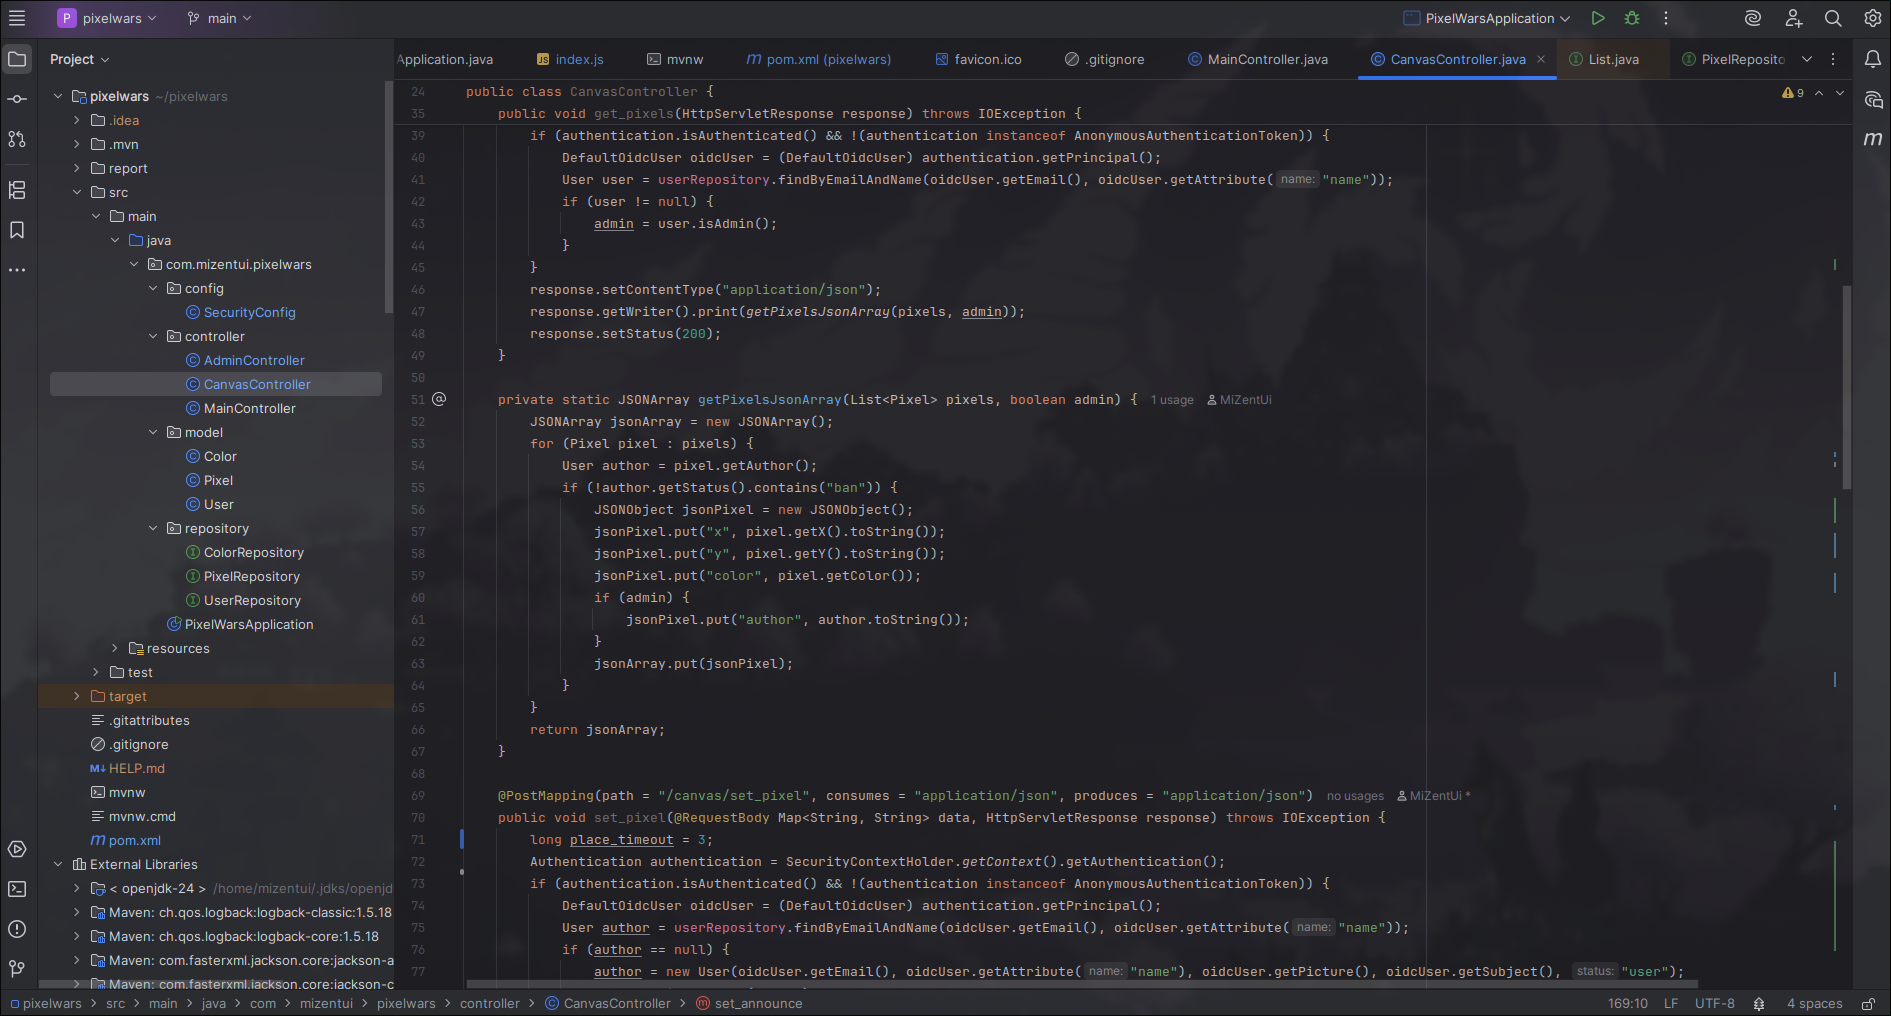
\includegraphics[width=\textwidth]{idea.png}
    \caption{Экран редактирования кода IntelliJ IDEA}
\end{figure}

IntelliJ IDEA — это интегрированная среда разработки (IDE), созданная компанией JetBrains для разработки программного обеспечения на языке Java и других языках платформы JVM. С момента своего появления в 2001 году, IntelliJ IDEA зарекомендовала себя как одна из наиболее мощных и удобных сред разработки, широко используемая в промышленной и академической практике. \cite{idea}

IntelliJ IDEA предоставляет полный набор инструментов, необходимых для создания современных Java-приложений, включая интеллектуальную навигацию по коду, рефакторинг, отладку, анализ производительности, тестирование и встроенную поддержку систем контроля версий. Среда активно поддерживает фреймворки, такие как Spring, Hibernate, Maven, Gradle и многие другие, что делает её особенно удобной при разработке серверной части сложных приложений.

В рамках курсового проекта IntelliJ IDEA использовалась для разработки серверной части системы Pixel Wars. Она обеспечила удобную интеграцию с фреймворком Spring Boot, возможность работы с базой данных PostgreSQL через встроенные плагины, а также автоматическую генерацию и управление зависимостями через систему сборки Gradle.

Причины выбора данной среды разработки включают:
\begin{enumerate}
    \item
          Глубокая интеграция с Java и Spring Boot. IntelliJ IDEA предоставляет интеллектуальную поддержку аннотаций, конфигурации и кода, специфичного для Spring, что значительно ускоряет процесс разработки.
    \item
          Автоматизация и интеллектуальные подсказки. Среда активно подсказывает доступные методы, проверяет корректность конфигураций, предлагает варианты рефакторинга и автоматически управляет импортами.
    \item
          Удобная работа с базой данных. Встроенные средства позволяют подключаться к PostgreSQL напрямую из среды, выполнять запросы, просматривать структуру таблиц и редактировать содержимое.
    \item
          Инструменты отладки и тестирования. IntelliJ IDEA содержит мощные инструменты для локальной отладки, трассировки выполнения и написания модульных тестов с использованием JUnit.
\end{enumerate}

Таким образом, использование IntelliJ IDEA обеспечило стабильную и эффективную среду для разработки серверной части проекта. Её функциональные возможности и адаптация под современные технологии Java сделали процесс создания приложения удобным, гибким и соответствующим промышленным стандартам.

\subsection{Среда разработки Visual Studio Code}

\begin{figure}[H]
    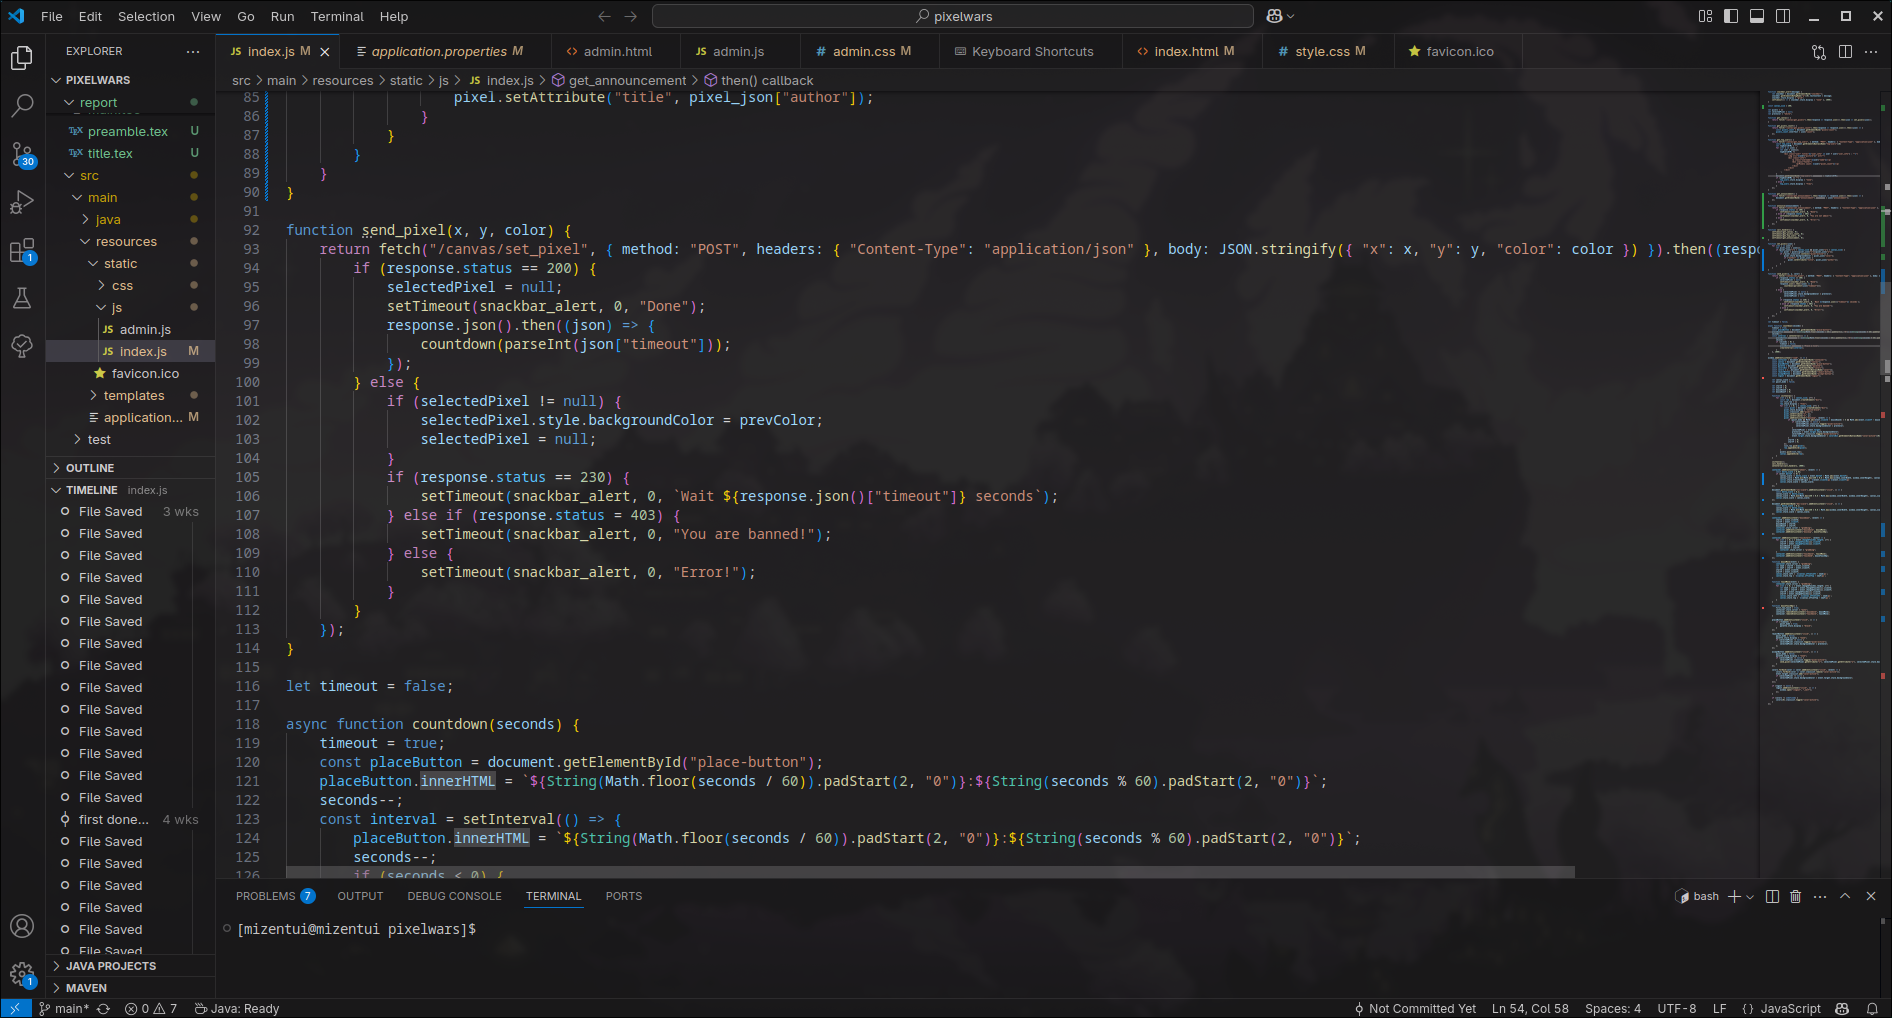
\includegraphics[width=\textwidth]{vscode.png}
    \caption{Экран редактирования кода Visual Studio Code}
\end{figure}

Visual Studio Code (VS Code) — это лёгкая, но мощная интегрированная среда разработки, разработанная компанией Microsoft. С момента своего выхода в 2015 году она завоевала огромную популярность благодаря простоте, быстроте и гибкости. VS Code является кроссплатформенным инструментом, доступным на Windows, macOS и Linux, что делает его универсальным решением для разработчиков по всему миру. \cite{vscode}

VS Code не перегружена лишними функциями, но в то же время предоставляет всё необходимое для разработки: интеллектуальную подсветку синтаксиса, автодополнение, отладку, поддержку Git, систему контроля версий и встроенный терминал. Это позволяет разрабатывать и тестировать код быстро и эффективно, без лишних задержек.

В проекте Pixel Wars Visual Studio Code использовалась для разработки фронтенда. Среда идеально подошла для создания клиентской части приложения, поскольку она поддерживает работу с JavaScript, HTML и CSS, а также позволяет интегрировать популярные фреймворки и библиотеки.

Основные причины выбора VS Code включают:
\begin{enumerate}
    \item
          Лёгкость и быстродействие. VS Code быстро запускается и работает с минимальными задержками, что делает её идеальной для разработки фронтенд-части и быстрого прототипирования.
    \item
          Расширяемость. Благодаря множеству доступных расширений, VS Code легко адаптируется под любые задачи. В проекте использовались расширения для работы с JavaScript, CSS, HTML, а также плагины для отладки и тестирования кода.
    \item
          Интеграция с Git и другими системами контроля версий. VS Code имеет встроенную поддержку Git, что упрощает работу с репозиториями и позволяет эффективно управлять версиями проекта.
\end{enumerate}

Visual Studio Code идеально подошла для разработки фронтенда Pixel Wars, предоставив удобные инструменты для работы с кодом, расширяемость и простоту в освоении. Весь процесс разработки клиентской части был значительно ускорен благодаря этой мощной и гибкой среде разработки. Даже этот документ написан в VS Code с использованием \LaTeX.

\subsection{Хостинг и развёртывание приложения}

\begin{figure}[H]
    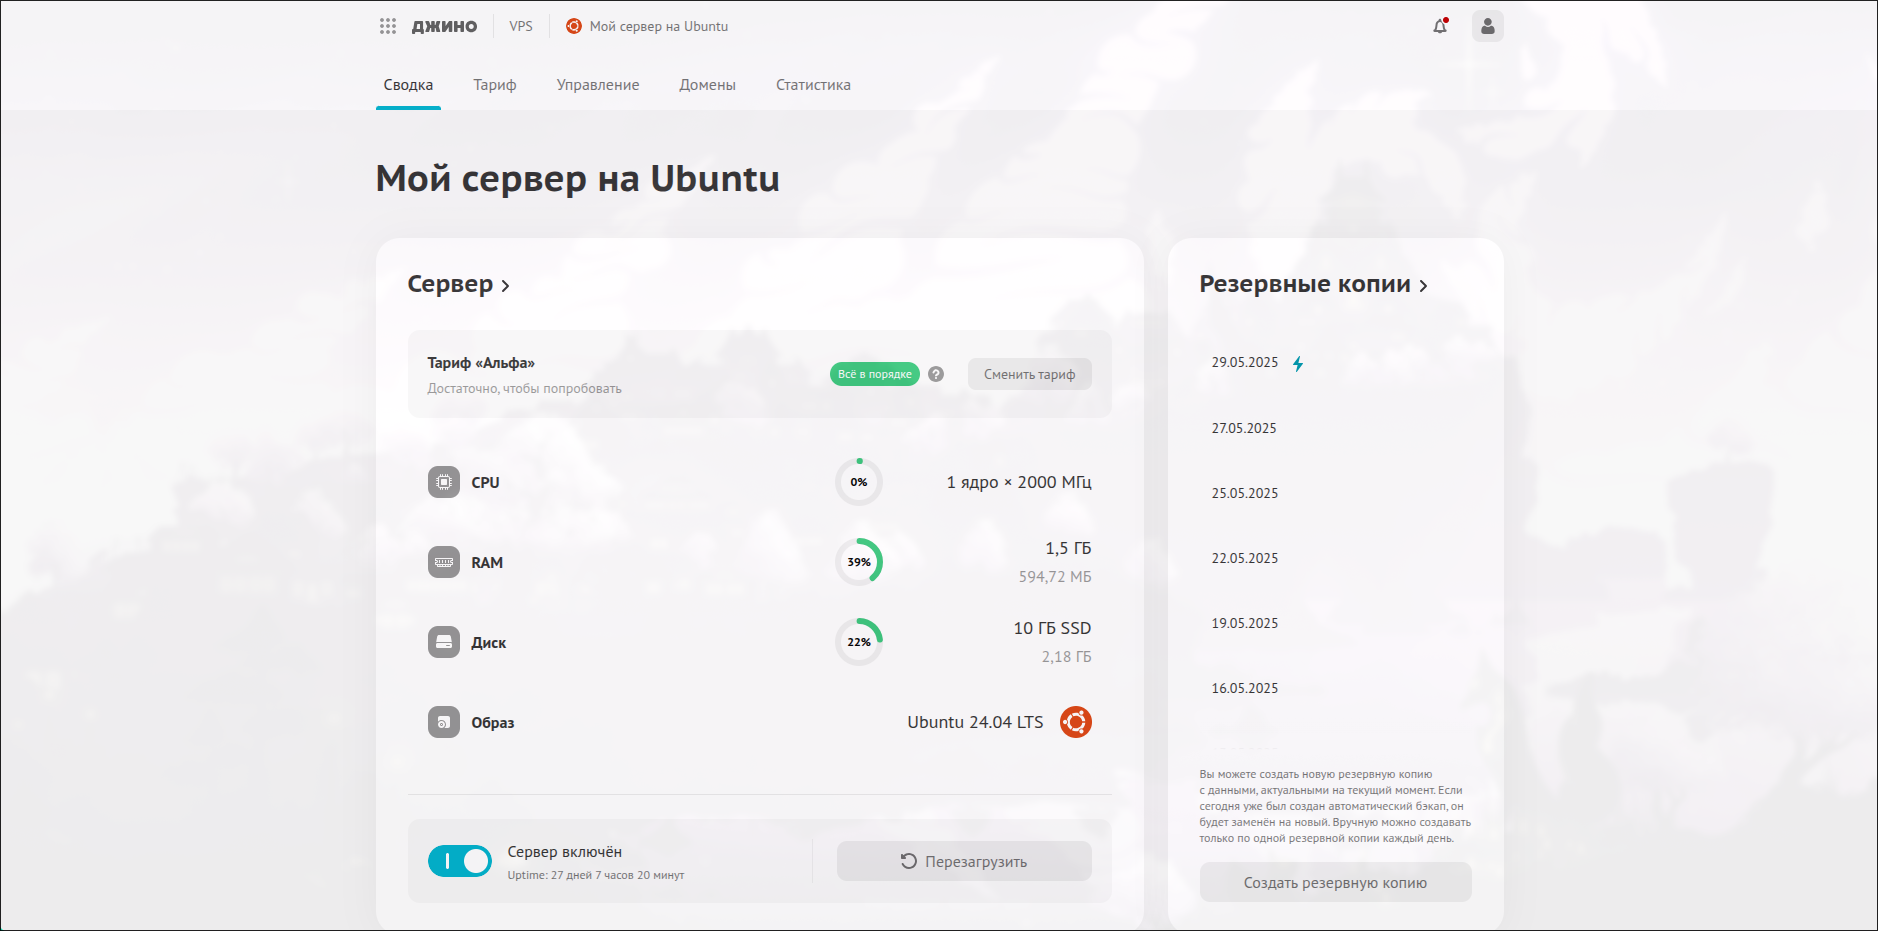
\includegraphics[width=\textwidth]{jino.png}
    \caption{Страница сервера на jino.ru}
\end{figure}

Для размещения серверной части проекта Pixel Wars использовался платный хостинг-провайдер Jino.ru. Выбор данного провайдера был обусловлен возможностью полного управления сервером через SSH-доступ, поддержкой системных сервисов, а также интеграцией доменов и SSL-сертификатов. \cite{jino}

Развёртывание приложения осуществляется на выделенный виртуальный сервер (VPS), работающий под управлением операционной системы Linux. Доступ к серверу выполняется с использованием безопасного протокола SSH, что позволяет выполнять все действия удалённо: загрузку файлов, настройку служб и управление серверной частью.

Сборка проекта осуществляется с использованием системы Maven. После успешной сборки на локальной машине создаётся JAR-файл, который загружается на сервер с помощью SCP. Развёртывание приложения производится вручную, без использования CI/CD, с контролем всех этапов.

Для автоматического запуска и надёжной поддержки работоспособности серверной части был создан отдельный systemd-сервис, зарегистрированный в системе как юнит. Этот сервис обеспечивает:
\begin{itemize}
    \item автоматический запуск приложения при загрузке сервера;
    \item перезапуск в случае сбоев;
    \item логирование через системный журнал.
\end{itemize}

Конфигурация systemd-юнита включает в себя путь к исполняемому JAR-файлу, указание рабочей директории, параметров Java-машины и стандартных параметров управления службой.

Для доступа к приложению по HTTPS был зарегистрирован собственный домен, приобретённый через панель управления Jino. К домену подключён wildcard-сертификат, позволяющий защищать не только основной домен, но и все его поддомены. Сертификат установлен на стороне веб-сервера, который при необходимости может проксировать запросы к приложению, обеспечивая безопасную и надёжную маршрутизацию трафика.


Использование Jino в качестве хостинг-платформы позволило обеспечить:
\begin{itemize}
    \item полную автономность и контроль над серверной средой;
    \item надёжную работу приложения в режиме 24/7;
    \item безопасный доступ пользователей по защищённому протоколу HTTPS;
    \item удобную интеграцию домена и сертификатов.
\end{itemize}

Развёртывание проекта в реальной среде подтвердило его работоспособность вне среды разработки и позволило провести полноценное тестирование функциональности в условиях, приближенных к промышленной эксплуатации.

\newpage

\sectionuppercase{Технические особенности реализации}

Данная глава посвящена описанию ключевых технических решений, реализованных в проекте.

\subsection{Обновление холста}

Механизм обновления холста в проекте Pixel Wars реализован на основе архитектуры клиент–сервер. Обновление инициируется на клиентской стороне с помощью HTTP-запроса к серверу, который возвращает актуальное состояние холста в формате JSON. Данные обрабатываются и визуализируются без необходимости перезагрузки страницы, обеспечивая плавную и интерактивную работу интерфейса.

Клиентская часть периодически отправляет GET-запрос на REST-эндпоинт, предназначенный для получения текущего состояния холста. В ответ сервер возвращает массив пикселей, каждый из которых содержит координаты и цвет. После получения ответа данные передаются в обработчик, который обновляет внешний вид холста на странице пользователя.

Серверная часть принимает запрос и формирует ответ, основываясь на данных, хранящихся в базе. Сначала извлекаются последние установленные пиксели для каждой координаты. Затем, при наличии активной авторизации, проверяется роль пользователя: если это администратор, в ответ дополнительно включается информация об авторах пикселей. Пиксели, установленные пользователями со статусом блокировки, фильтруются и не включаются в выдачу.

Ответ формируется в формате JSON и отправляется клиенту с указанием соответствующего типа контента.

После получения ответа клиентская часть обрабатывает каждый пиксель: проверяется его позиция и текущее состояние на экране. Если пиксель ранее не был обновлён, ему присваивается цвет, полученный от сервера. В случае если пользователь имеет административные права, к пикселю добавляется всплывающая подсказка с именем автора.

В результате реализованная система позволяет:
\begin{itemize}
    \item отображать актуальное состояние холста всем пользователям;
    \item разграничивать доступ к дополнительной информации (например, авторам пикселей) в зависимости от роли;
    \item динамически обновлять интерфейс без полной перезагрузки страницы.
\end{itemize}

\subsection{Установка пикселя на холст}

Механизм установки пикселя реализован с использованием REST-запросов. Пользователь, взаимодействуя с холстом, выбирает координаты и цвет, после чего инициирует отправку запроса на сервер для фиксации результата. Это обеспечивает динамичное взаимодействие без полной перезагрузки страницы и позволяет достичь высокой отзывчивости пользовательского интерфейса.

На стороне клиента формируется POST-запрос, содержащий следующие данные:
\begin{itemize}
    \item координаты пикселя (x, y);
    \item цвет в формате RGB или HEX;
    \item тело запроса в формате JSON.
\end{itemize}

Запрос направляется на соответствующий серверный эндпоинт, где происходит последовательная обработка.

Во-первых, осуществляется проверка аутентификации пользователя. Затем проверяется статус доступа. В случае блокировки (например, статус \texttt{ban}) сервер отклоняет запрос с кодом состояния 403 (Forbidden).

Во-вторых, применяется ограничение по времени между действиями. Сервер анализирует историю пикселей, размещённых пользователем, и вычисляет, сколько времени прошло с момента последнего действия. Если минимальный интервал ещё не истёк, сервер возвращает специальный код 230 и значение оставшегося времени ожидания.

Если все условия соблюдены (пользователь авторизован, не заблокирован и не нарушает временные ограничения), сервер сохраняет пиксель в базу данных.

Вносятся следующие параметры:
\begin{itemize}
    \item координаты: x, y;
    \item цвет пикселя;
    \item временная метка;
    \item идентификатор пользователя.
\end{itemize}

В ответ клиент получает JSON-объект, содержащий:
\begin{itemize}
    \item статус выполнения (успешно или с ошибкой);
    \item значение таймера \texttt{timeout}, определяющее задержку до следующего действия.
\end{itemize}

После получения ответа клиентская часть:
\begin{itemize}
    \item запускает таймер обратного отсчёта;
    \item временно блокирует интерфейс взаимодействия с холстом;
    \item в случае ошибки выводит уведомление о причине отказа (ожидание, запрет доступа, общая ошибка).
\end{itemize}

Таким образом, установка пикселя реализована как контролируемая операция с учётом аутентификации и ролевой модели. Данная архитектура позволяет обеспечить стабильную и безопасную механику многопользовательского взаимодействия.

\subsection{Система модерации и панель администратора}

\begin{figure}[!h]
    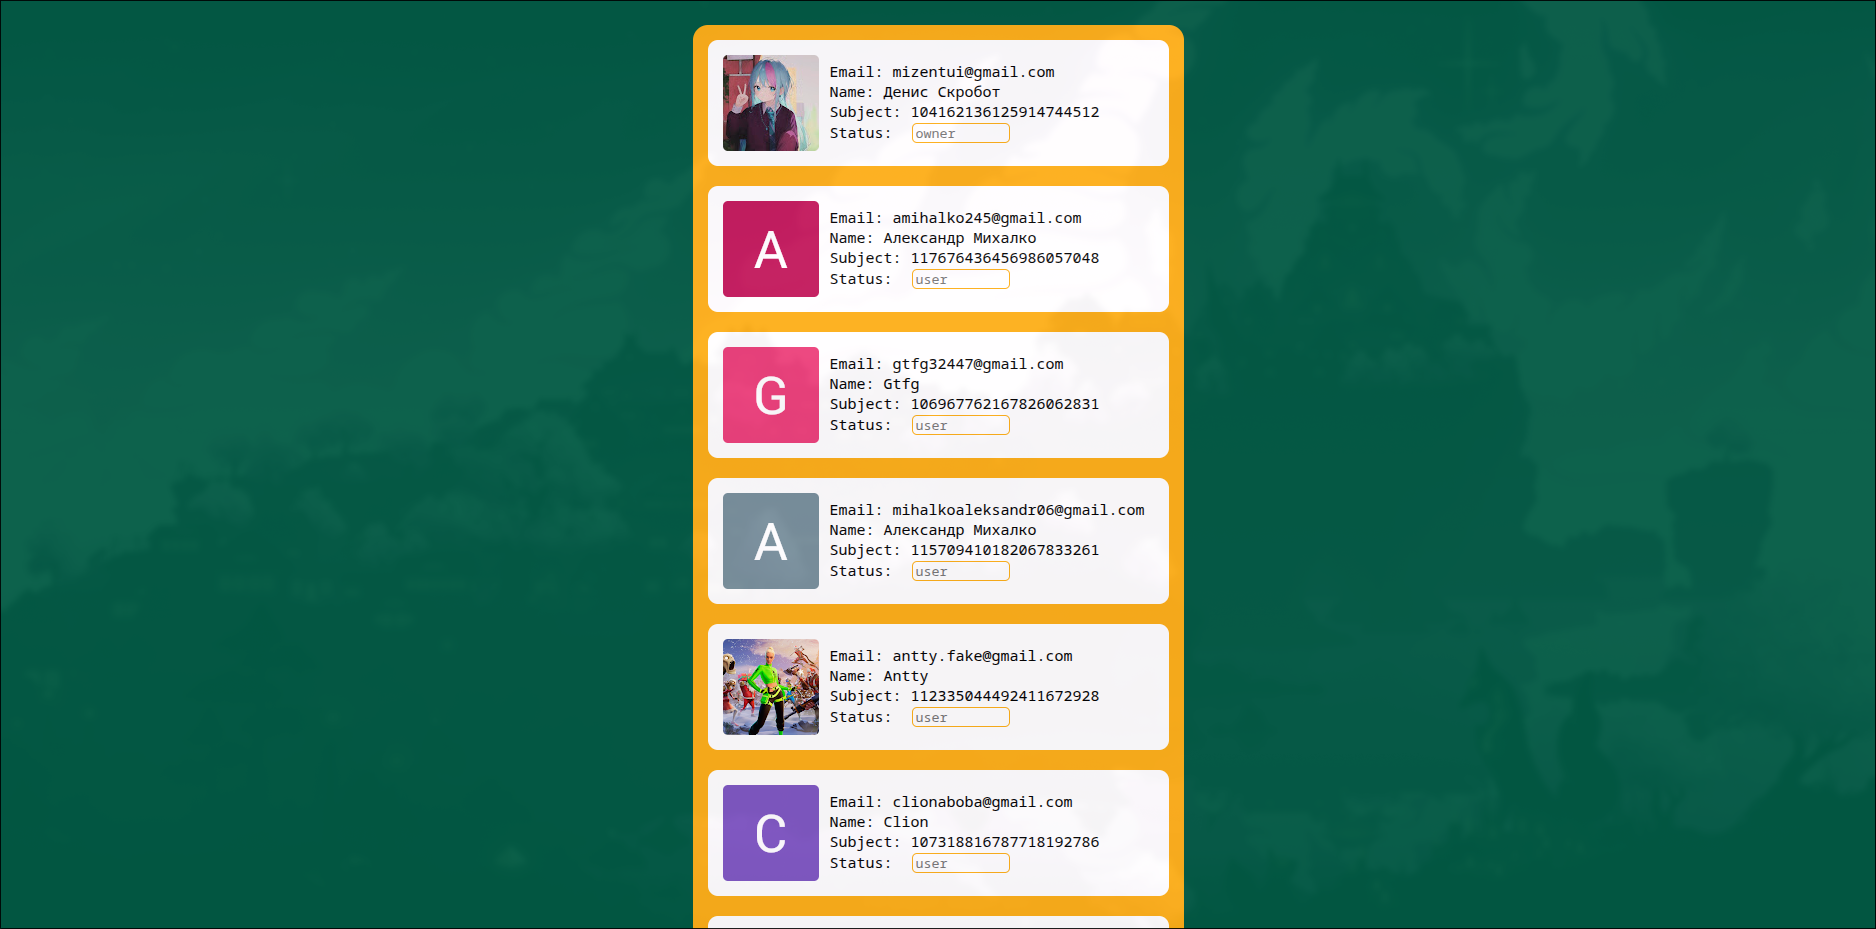
\includegraphics[width=\textwidth]{admin.png}
    \caption{Интерфейс панели администратора}
\end{figure}

Для обеспечения контроля за поведением пользователей и соблюдением игровых правил в проекте Pixel Wars реализована система модерации, доступ к которой имеет только администратор. Административные функции включают просмотр всех зарегистрированных пользователей, изменение их статусов и блокировку нарушителей.

Модерация реализована через отдельный REST-контроллер серверной части, доступ к которому ограничен на уровне авторизации. При входе в административный интерфейс, если пользователь обладает статусом администратора, он получает доступ к следующему функционалу:
\begin{itemize}
    \item просмотр списка всех зарегистрированных пользователей;
    \item отображение основной информации о каждом пользователе (имя, email, subject, статус, изображение профиля, количество установленных пикселей);
    \item возможность изменить статус пользователя.
\end{itemize}

На стороне клиента административная панель реализована в виде отдельного интерфейсного блока, который динамически запрашивает список пользователей с сервера. Для этого используется периодическая отправка GET-запросов на серверный эндпоинт, обрабатываемый соответствующим контроллером. При получении ответа в формате JSON информация обновляется на странице без перезагрузки.

При изменении статуса конкретного пользователя (например, перевод в статус \texttt{ban} или \texttt{admin}) отправляется POST-запрос с указанием идентификатора пользователя и нового статуса. Сервер проверяет авторизацию текущего пользователя, наличие прав администратора и допустимость изменения (в частности, невозможно изменить статус пользователей со статусом «owner»). После успешного обновления информации клиент получает подтверждение и обновлённый список пользователей.

Для визуальной обратной связи используется система уведомлений, реализованная в виде всплывающего блока. Пользователь получает сообщение о результате операции: успешно ли изменён статус или произошла ошибка.

Список возможных статусов:
\begin{itemize}
    \item \texttt{owner} --- статус владельца --- привилегии как у \texttt{admin}, но не возможно инзменить статус владельцу через панель администратора;
    \item \texttt{admin} --- статус администратора --- может менять статус другим пользователям, кроме владельца, также заходить в панель администратора и просматривать данные пользователей;
    \item \texttt{creator} --- статус художника --- может ставить пиксели без временного ограничения;
    \item \texttt{user} --- статус пользователя;
    \item \texttt{ban} --- статус блокировки --- пользователь не может рисовать и поставленные ранее пиксели не отображаются на общем холсте.
\end{itemize}

Система модерации предоставляет администратору инструменты для управления пользовательской активностью, контроля за соблюдением правил, блокировки нарушителей на платформе. Простота реализации и интуитивный интерфейс позволяют эффективно использовать административные функции даже без технической подготовки.

\newpage

\sectionuppercase{Тестирование}

Тестирование проекта Pixel Wars проводилось поэтапно с постепенным расширением аудитории. Такой подход позволил выявить ключевые проблемы на ранних стадиях и обеспечить стабильную работу приложения при высокой нагрузке.

\textbf{Ручное тестирование.} На первом этапе тестирование выполнялось в ручном режиме непосредственно разработчиком. Проверялись базовые функции: установка пикселя, обновление холста, авторизация, система ограничения по времени, работа административной панели. Выявленные ошибки включали некорректную обработку исключений, нарушения в логике работы с таймерами, а также визуальные баги в интерфейсе.

\textbf{Тестирование с участием небольшой группы пользователей.} На втором этапе была подключена небольшая группа из 4 человек, которые моделировали реальное поведение пользователей: взаимодействовали с холстом, пробовали нарушить ограничения, отправляли частые запросы с разных устройств и браузеров. Это позволило проверить устойчивость системы при одновременных действиях и протестировать серверную нагрузку в условиях близких к реальным.

\textbf{Публикация проекта для широкой аудитории.} Финальный этап тестирования проходил в условиях реального использования. Проект был размещён на удалённом сервере и открыт для студентов БГУИР — общее количество пользователей составило около 50 человек. За 5 дней активного взаимодействия с холстом участники оставили множество изображений и надписей. Это позволило оценить, как приложение работает при нагрузке, а также получить обратную связь от реальных пользователей.

В ходе тестирования были выявлены и устранены следующие проблемы:
\begin{itemize}
    \item ошибки, связанные с блокировкой пользователей и логикой смены статуса;
    \item нестабильная работа timeout-механизма;
    \item высокая нагрузка на клиент при масштабном обновлении холста;
    \item недоработки в панели администратора.
\end{itemize}

В результате был собран полноценный холст, демонстрирующий коллективную активность. На нём присутствуют рисунки и другие элементы, созданные пользователями за время публичного тестирования.

\newpage
\clearpage

\begin{figure}[!ht]
    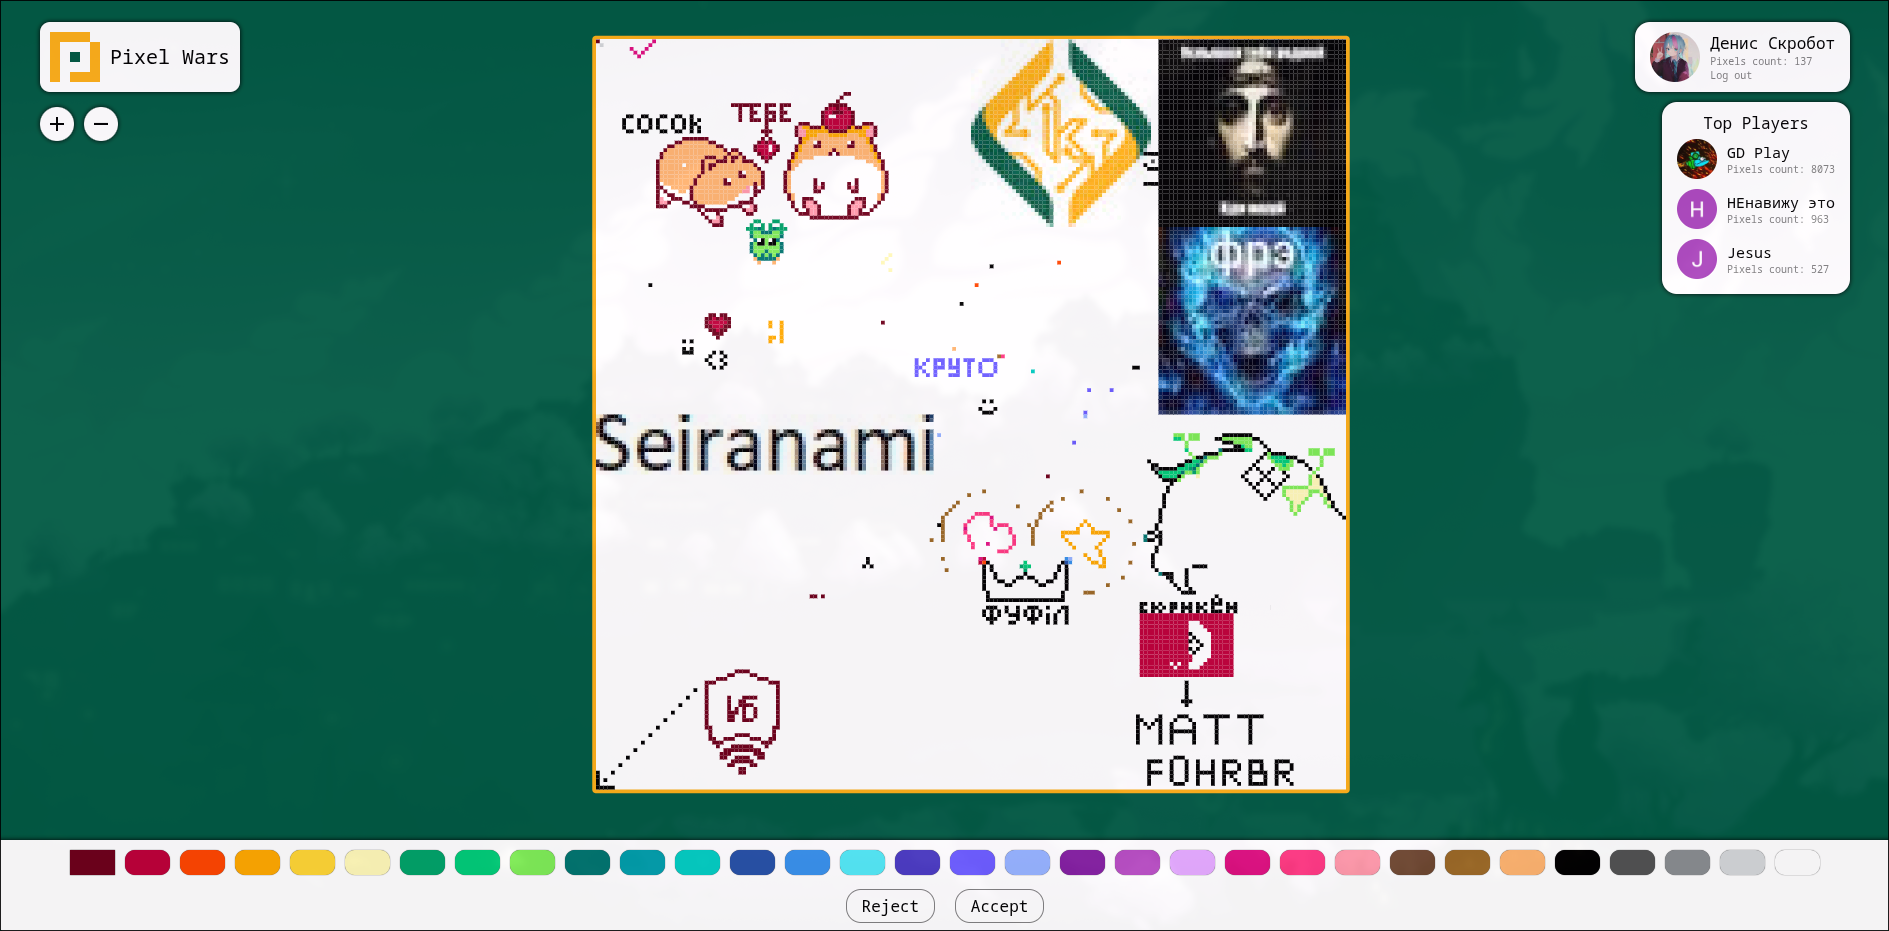
\includegraphics[width=\textwidth]{pixelwars.png}
    \caption{Интерфейс и холст Pixel Wars}
\end{figure}

\newpage

\addcontentsline{toc}{section}{Заключение}
\section*{\centering{\uppercase{Заключение}}}

В рамках данного курсового проекта была разработана многопользовательская онлайн-игра Pixel Wars, представляющая собой цифровой холст для коллективного рисования в реальном времени. Основной целью проекта было создание функционального, устойчивого и масштабируемого приложения, способного объединить большое количество пользователей в общем интерактивном пространстве.

Основные результаты и выводы:
\begin{enumerate}
    \item
          \textbf{Реализация клиент-серверной архитектуры.} Приложение построено по принципу разделения клиентской и серверной частей. Серверная часть реализована на Java с использованием Spring Boot, PostgreSQL. Клиент взаимодействует с сервером через REST-интерфейс, обеспечивая передачу данных о пикселях и состояниях пользователей.
    \item
          \textbf{Механизм управления холстом.} Разработан механизм установки пикселей с учётом ограничения по времени, фильтрации действий заблокированных пользователей и отображения авторов рисунков для администраторов.
    \item
          \textbf{Панель администратора и система модерации.} В системе реализован модуль управления пользователями. Администратор может просматривать информацию о пользователях, изменять их статус, а также отслеживать активность на холсте.
    \item
          \textbf{Полноценное тестирование и развёртывание.} Проект прошёл три этапа тестирования: ручное, с привлечением небольшой фокус-группы, и широкое публичное тестирование с участием около 50 студентов. В результате удалось собрать обратную связь, выявить и устранить ряд недочётов.
\end{enumerate}


Разработка данного проекта позволила углубить знания в области веб-технологий, серверной архитектуры, работы с базами данных, а также познакомиться с практикой проектирования и защиты распределённых систем. Были освоены современные подходы к реализации авторизации, разграничению прав доступа и синхронизации клиентской и серверной логики.

Таким образом, проект Pixel Wars стал не только учебным, но и практически значимым решением, подтвердившим свою работоспособность в реальной среде. Он заложил основу для дальнейшего развития и масштабирования: расширения функциональности, внедрения новых игровых механик, улучшения производительности и визуальной составляющей. Полученный мною опыт может быть использован в будущих проектах, связанных с созданием интерактивных многопользовательских приложений.